\subsection{External Interfaces}
\subsubsection{User Interfaces}

\begin{figure}[htbp]
    \centering
    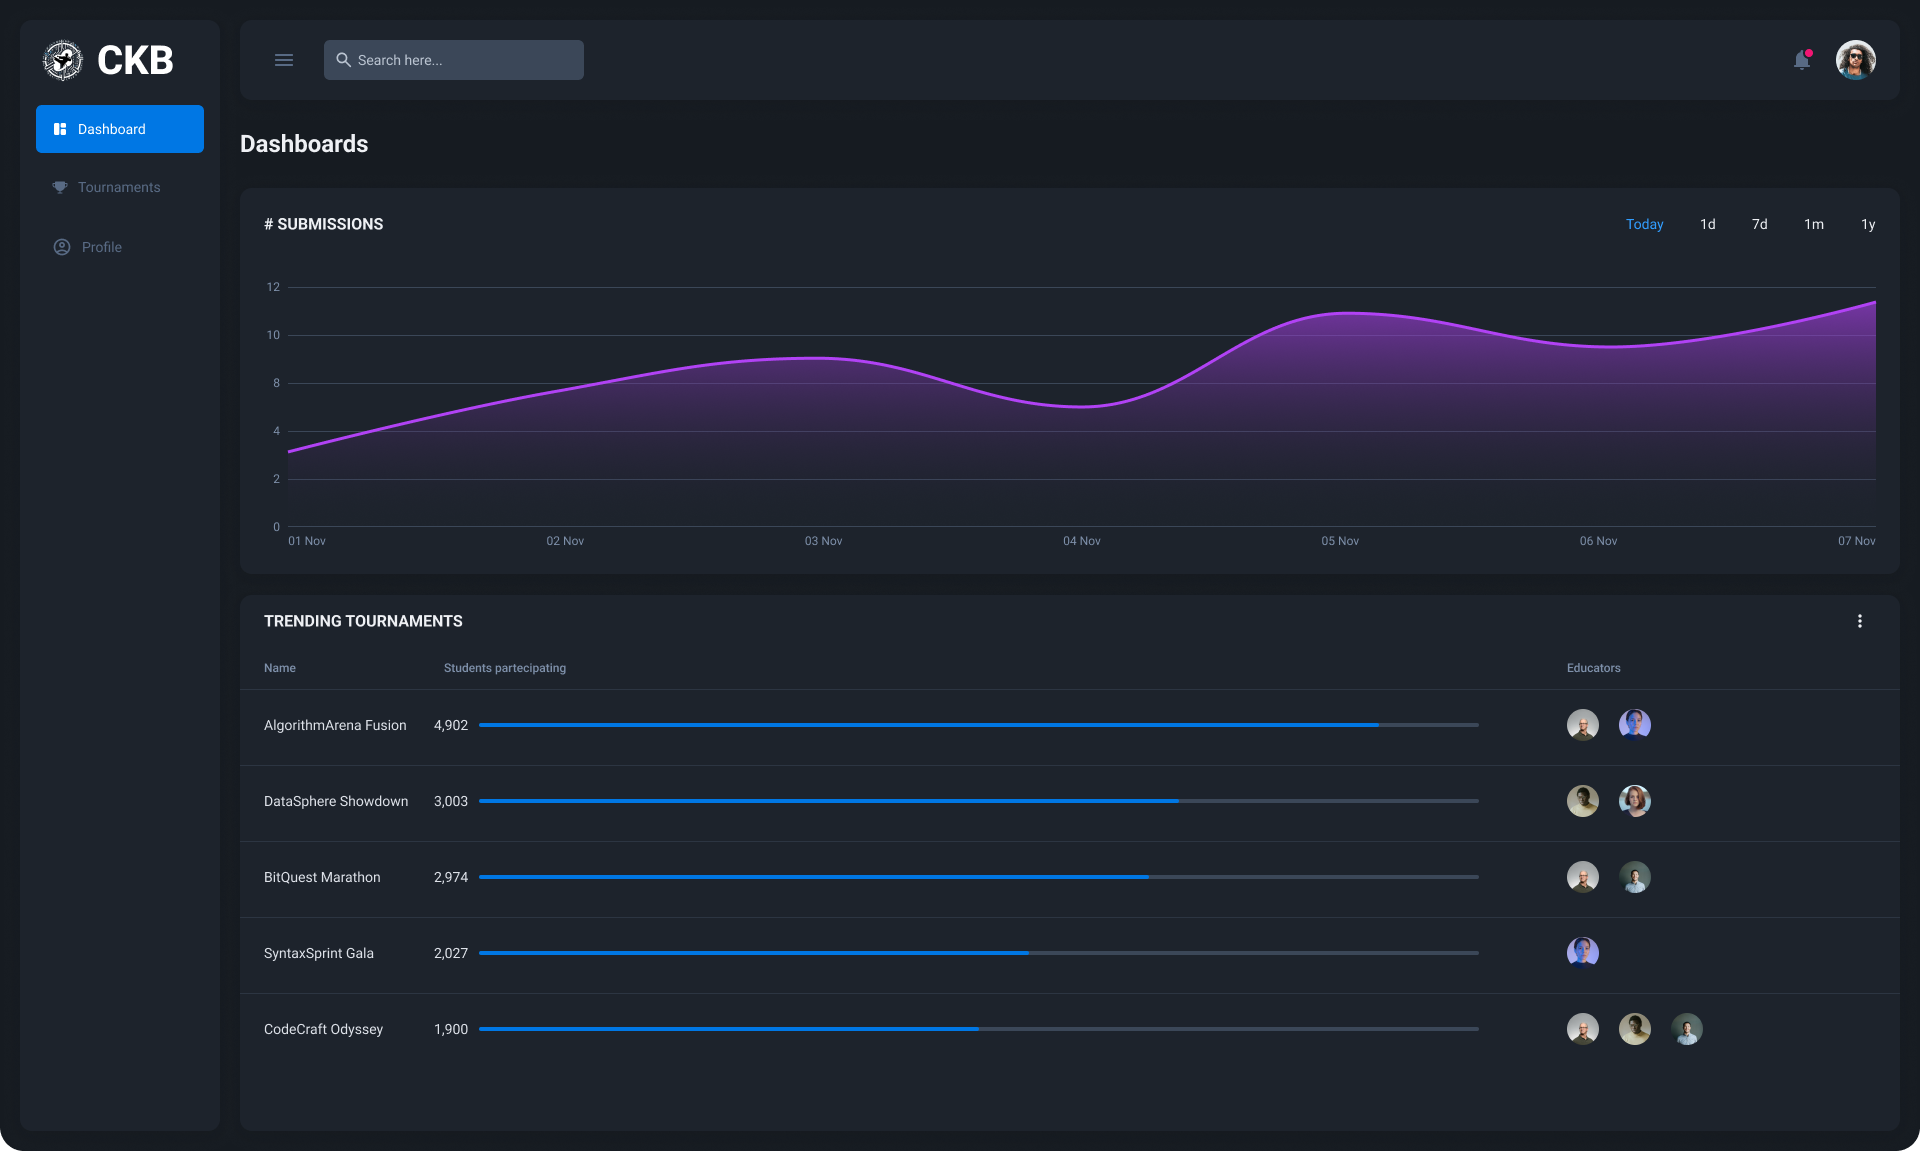
\includegraphics[width=\textwidth]{Images/Dashboard-Student.png}
    \caption{Student Dashboard}
    \label{fig:student-dashboard}
\end{figure}

\begin{figure}[htbp]
    \centering
    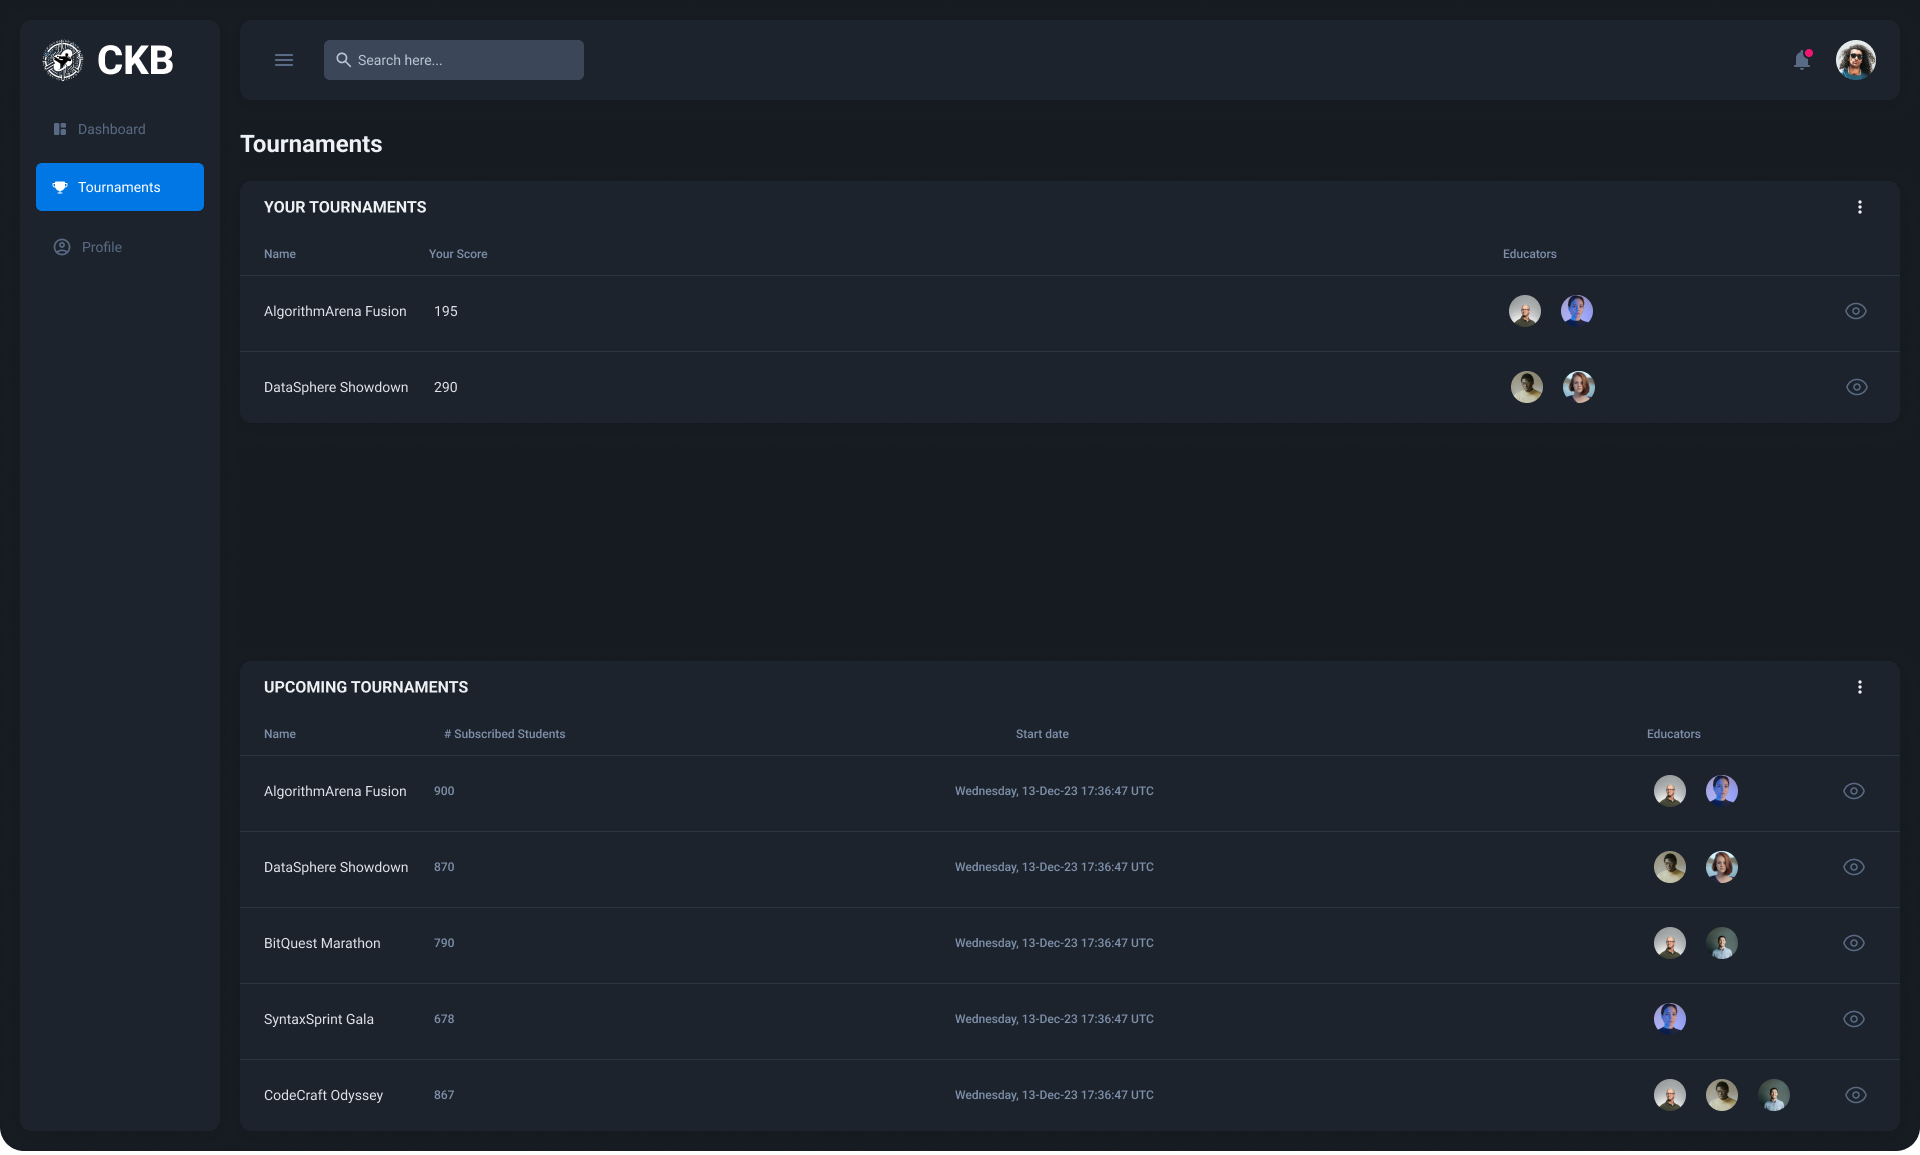
\includegraphics[width=\textwidth]{Images/Dashboard-Tournament.png}
    \caption{Student Dashboard Tournaments Tab}
    \label{fig:student-dashboard-tournaments}
\end{figure}

\begin{figure}[htbp]
    \centering
    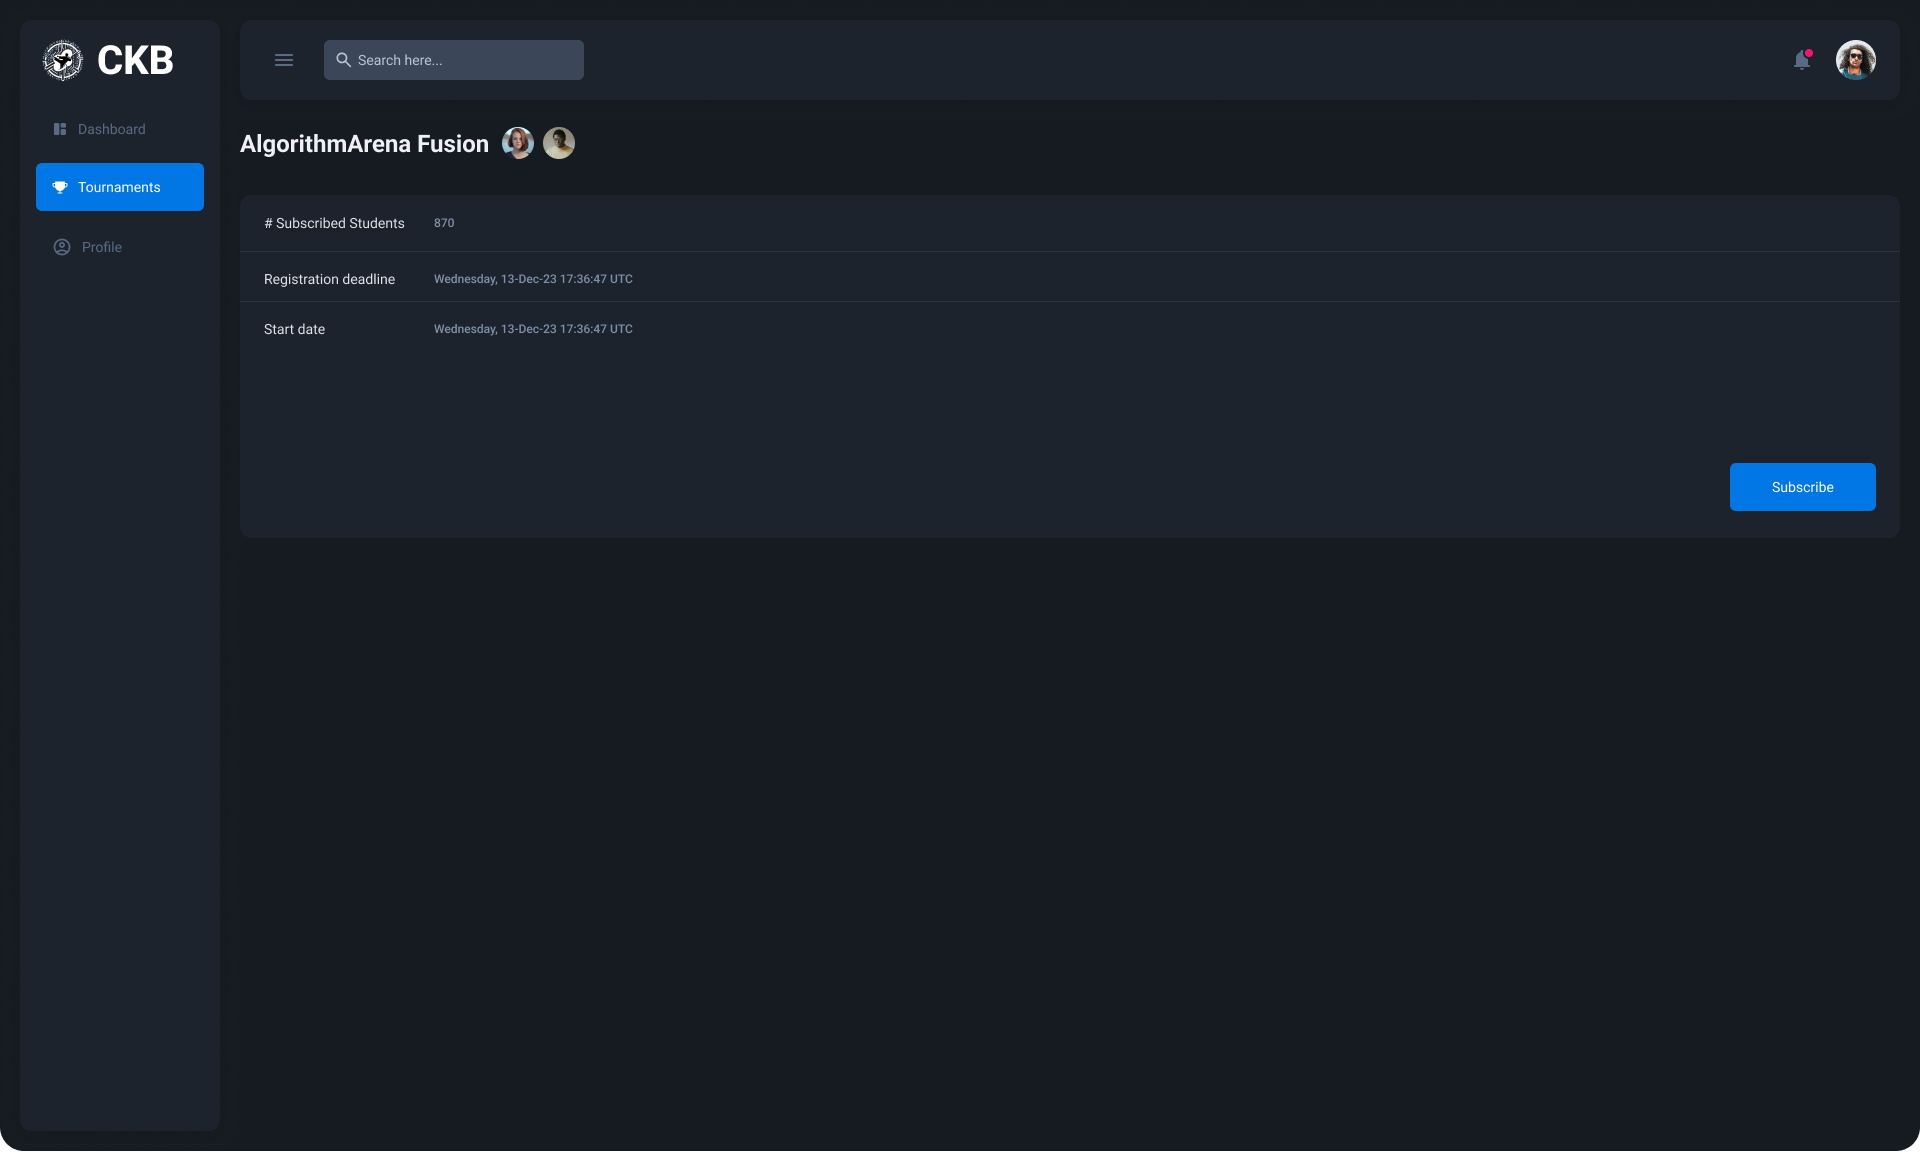
\includegraphics[width=\textwidth]{Images/Dashboard-Tournament-OverView.png}
    \caption{Student Dashboard Tournament OverView}
    \label{fig:student-Tournament-OverView}
\end{figure}

\begin{figure}[htbp]
    \centering
    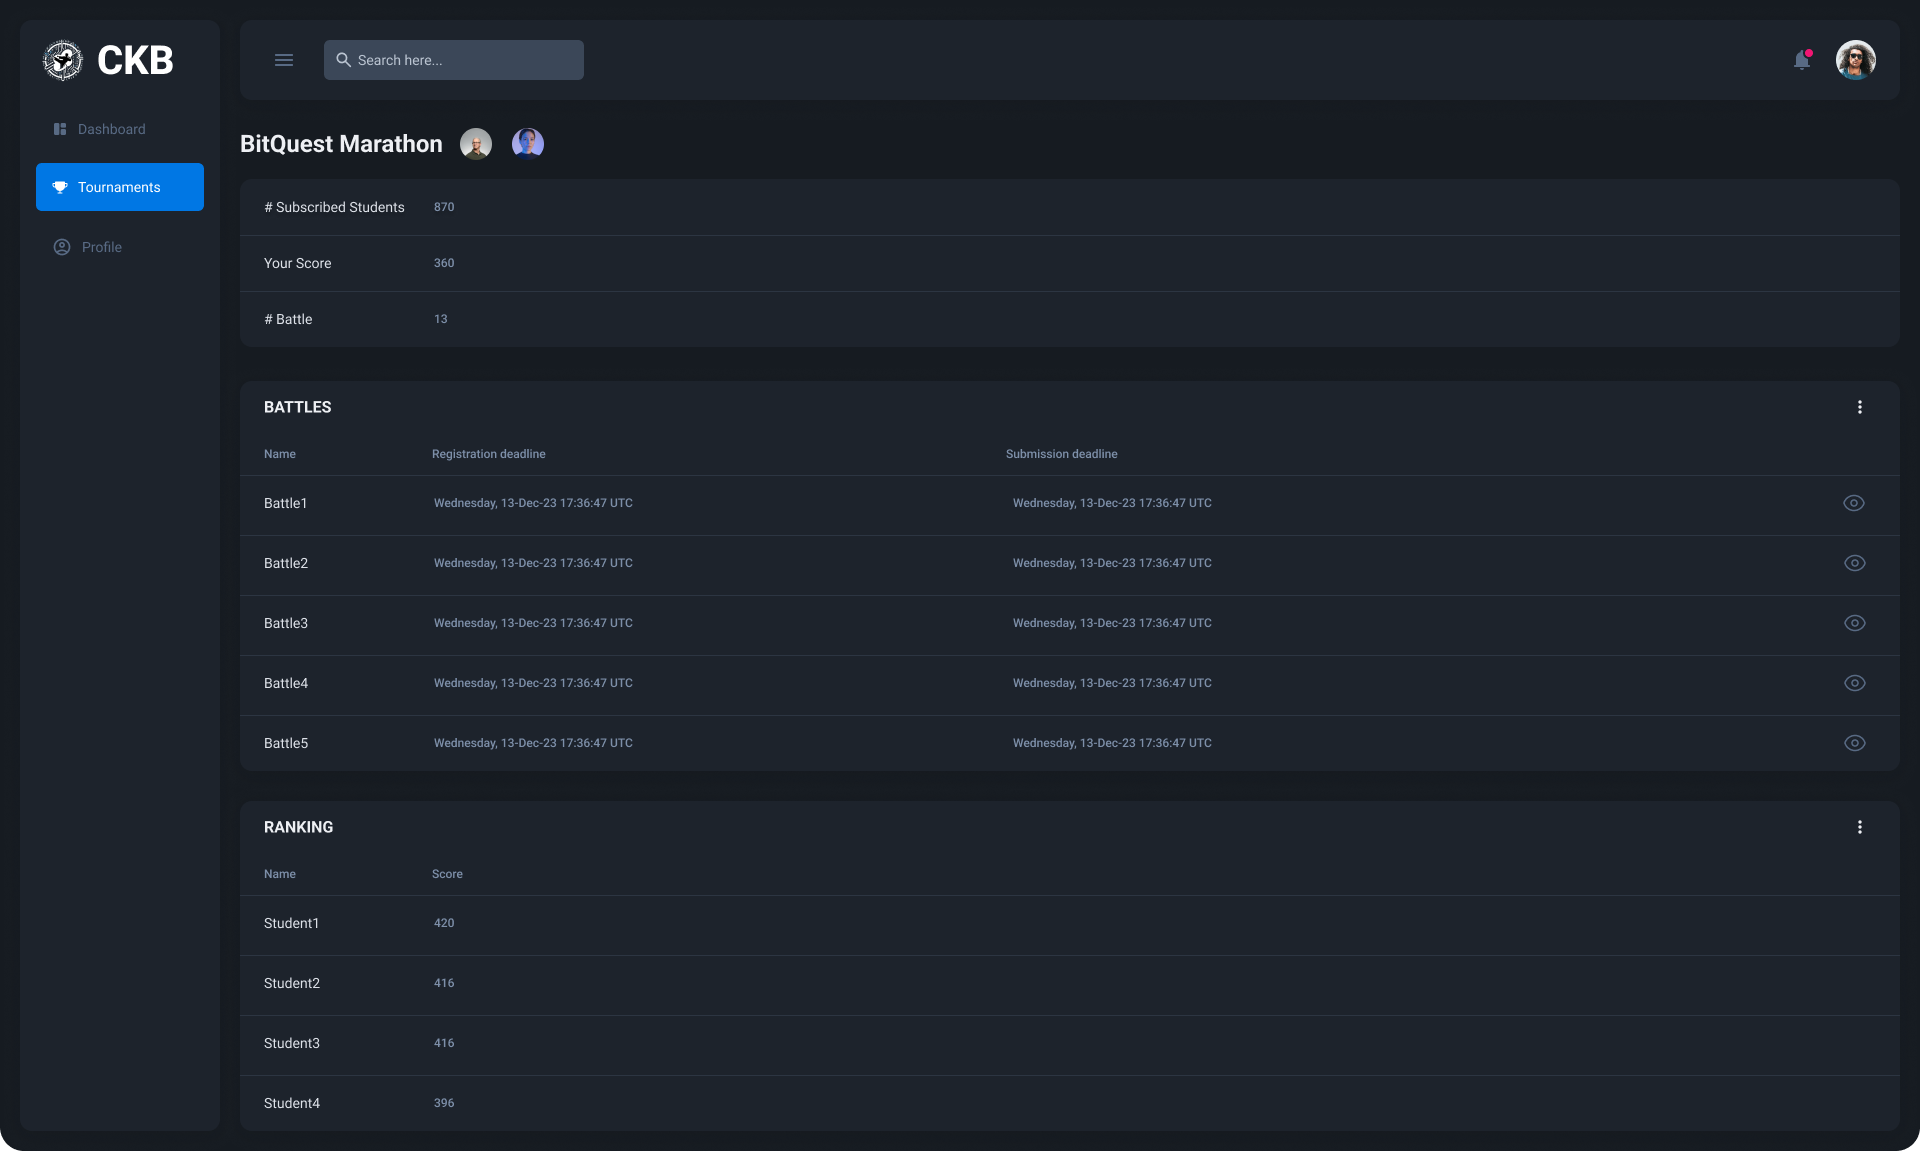
\includegraphics[width=\textwidth]{Images/Dashboard-Tournament-Ongoing.png}
    \caption{Student Dashboard Tournament Ongoing}
    \label{fig:student-Tournament-Ongoing}
\end{figure}

\begin{figure}[htbp]
    \centering
    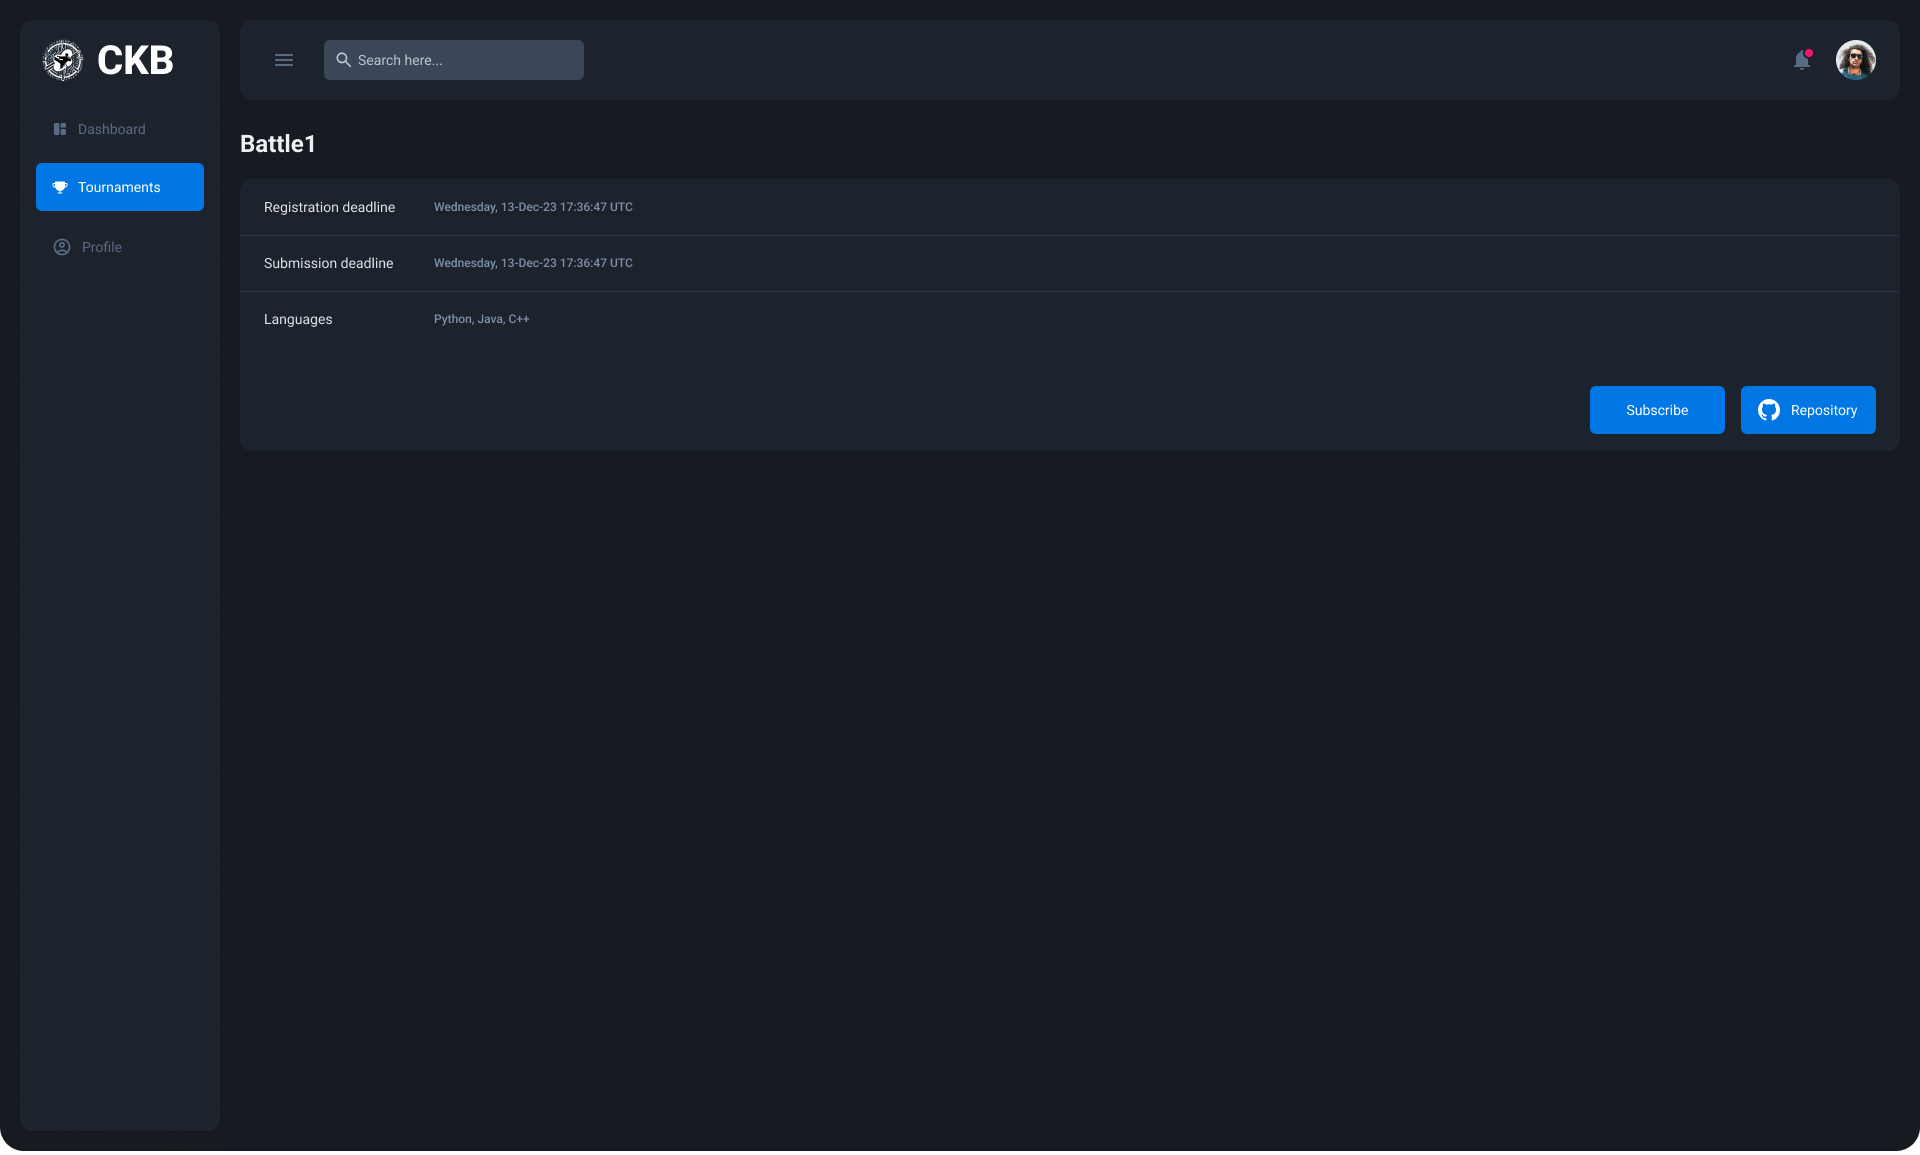
\includegraphics[width=\textwidth]{Images/Dashboard-Battle-Overview.png}
    \caption{Student Dashboard Battle Overview}
    \label{fig:student-Tournament-Completed}
\end{figure}


\subsubsection{Hardware Interfaces}
Since there is no particular hardware requirement for the system, the system will be able to run on any hardware that can run a web browser and has an internet connection.

\subsubsection{Software Interfaces}
The system in order to perform its functions does not require any interaction with other software systems.

\subsubsection{Communication Interfaces}
The system provides the functionality of automatic evaluation. This function requires the system to communicate with an external client that triggers this automatic actions. In particular, the system needs to expose an API that the GitHub Action set up by the students will call when a new commit is pushed.

\subsection{Functional Requirements}
This section specifies all the requirements that the system must satisfy in order to be considered complete and functional.

\begin{enumerate}[label=R\arabic*:]
    \item The system shall allow the user to register to the system
    \item The system shall allow the user to login to the system
    \item The system shall allow the educator to create a new tournament
    \item The system should allow the educator to create a new battle for a tournament
    \item The system shall allow the student to subscribe to a tournament
    \item The system shall allow the student to subscribe to a battle
    \item The system shall create a repository for each battle such that is forkable by the students
    \item The system shall allow the student to create a team for a battle
    \item The system should allow the student to invite other students to join a team
    \item The system should notify students subscribed to the platform when a new tournament is created
    \item The system should notify students subscribed to a tournament when a new battle is created
    \item The system should notify students subscribed to a tournament when the system publishes the ranking of the tournament
    \item The system shall guarantee that the restrictions for a battle set by the educator are respected
    \item The system shall allow the educator to set the restrictions for a battle
    \item The system shall allow the educator that created a tournament to invite other educators to the tournament
    \item The system shall allow the educator to close a tournament
    \item The system should allow the educator to manually update the score of a team for a battle
\end{enumerate}

\subsubsection{Use Cases Diagram}
\subsubsection*{Educator Use Diagram}
\begin{figure}[htbp]
    \centering
    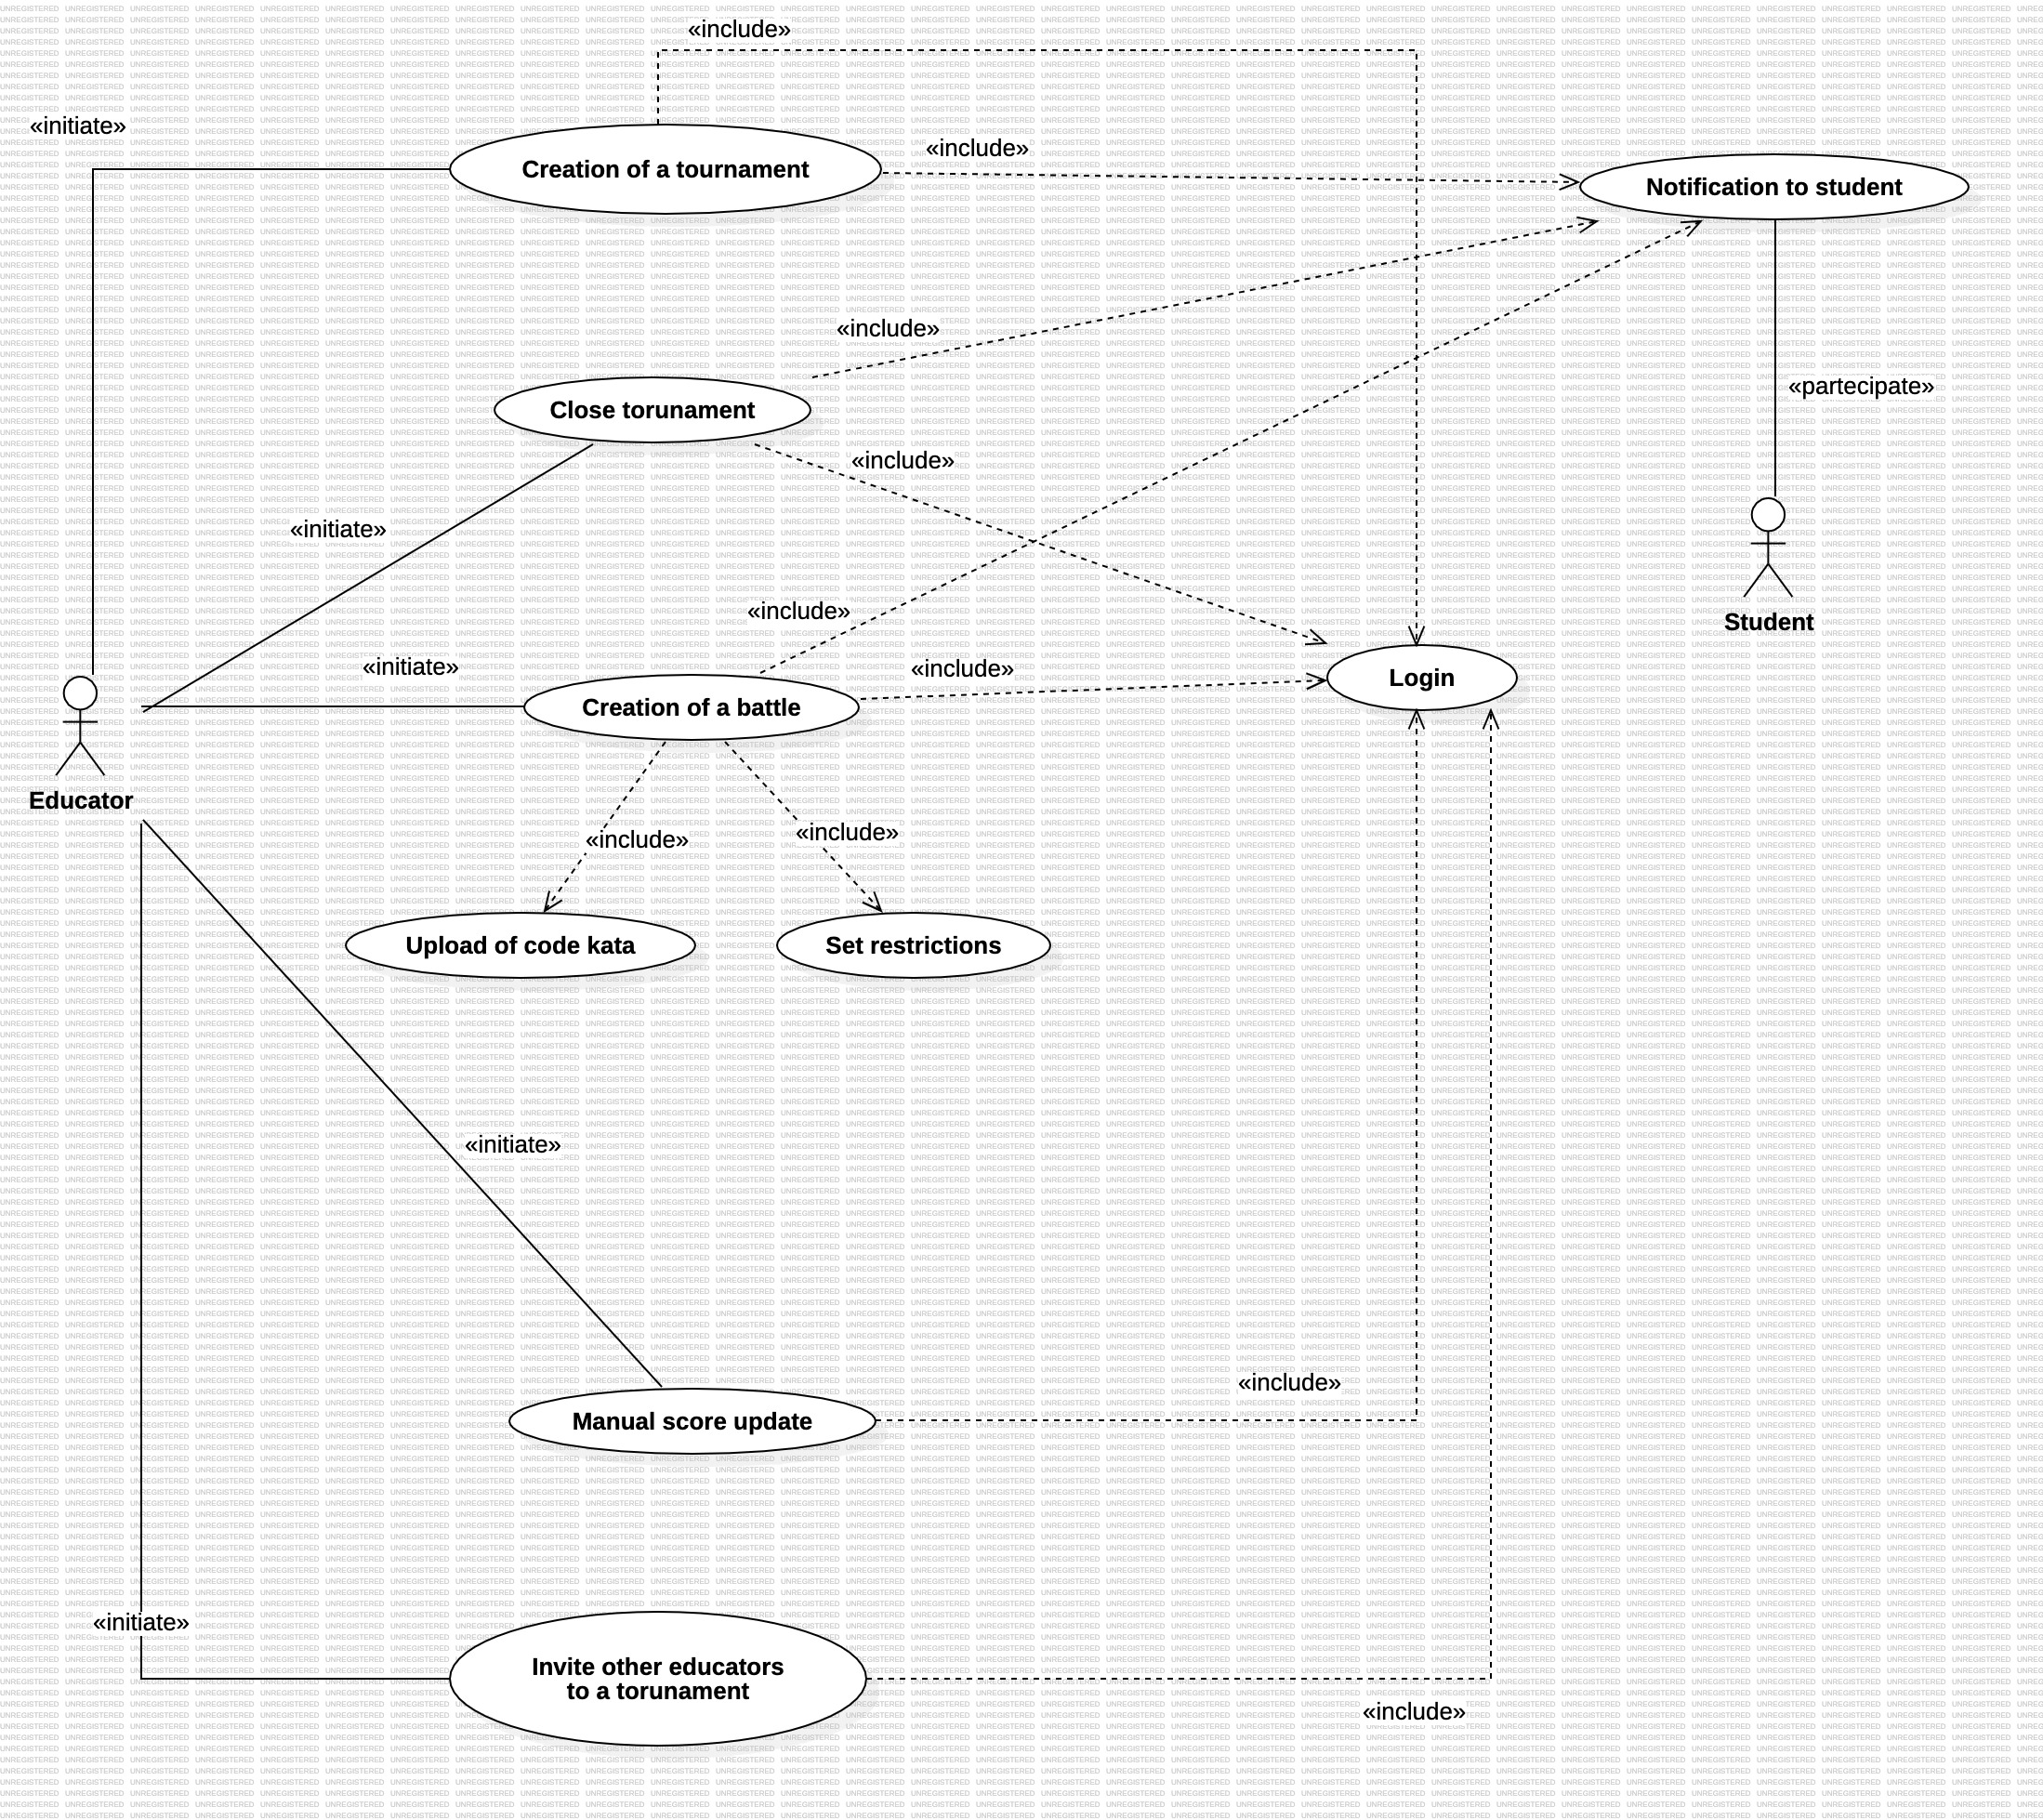
\includegraphics[width=\textwidth]{Diagrams/EducatorUseCaseDiagram.jpg}
    \caption{Educator Use Cases Diagram}
    \label{fig:student-use-diagram}
\end{figure}

\subsubsection*{Student Use Diagram}
\begin{figure}[htbp]
    \centering
    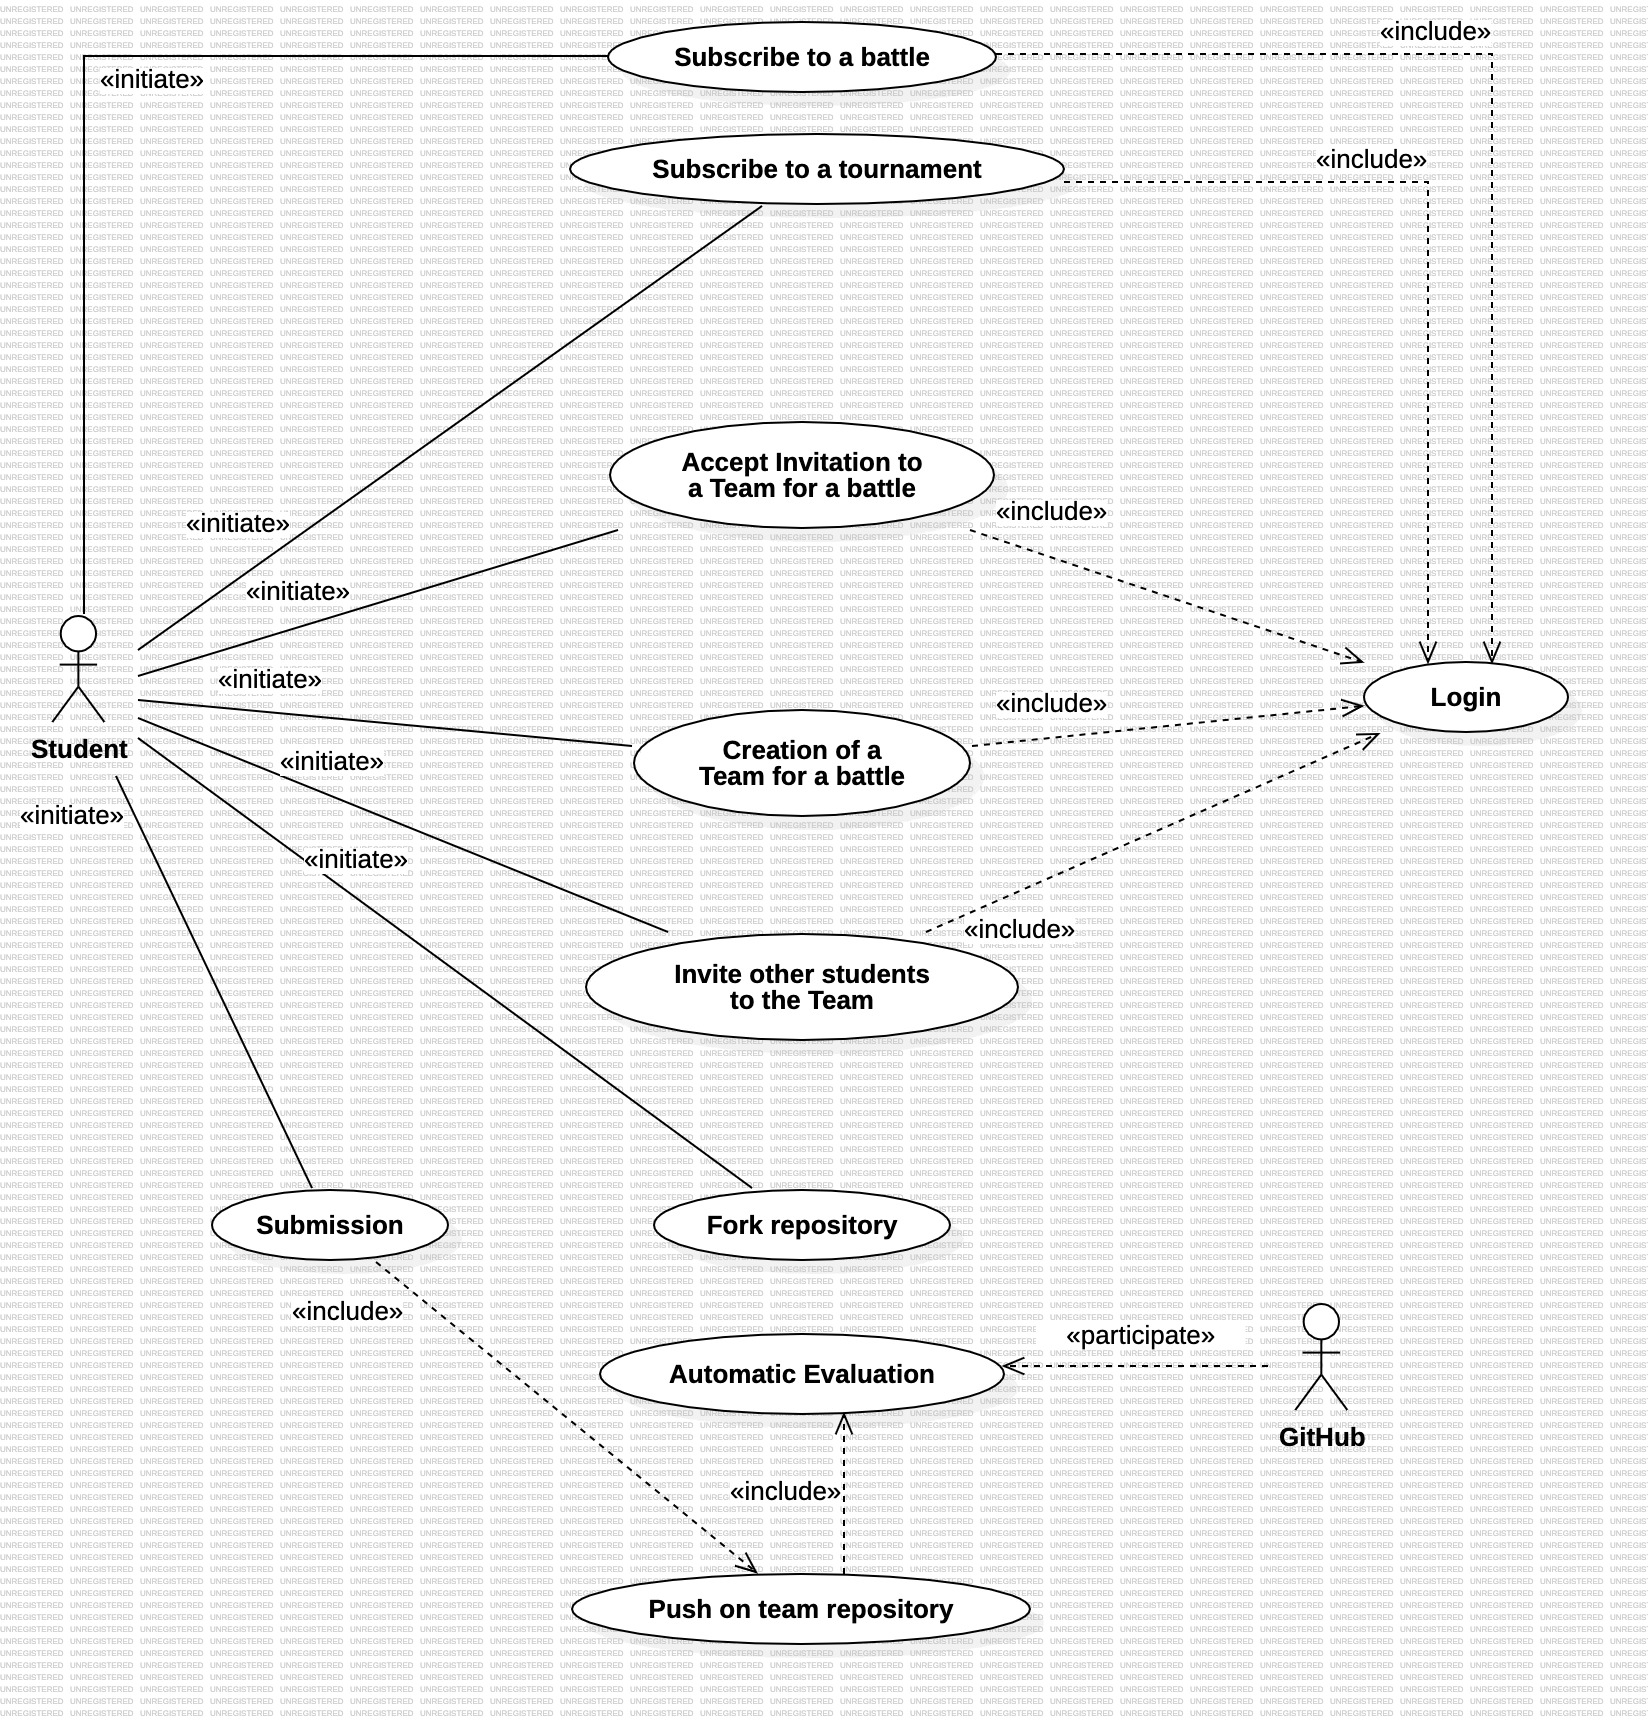
\includegraphics[width=\textwidth]{Diagrams/StudentUseCaseDiagram.jpg}
    \caption{Student Use Cases Diagram}
    \label{fig:student-use-diagram}
\end{figure}